\section{Auswertung}
\label{sec:Auswertung}
\subsection{Untersuchung des Acrylblocks mit einer Schieblehre}
Die Bohrungen des Acrylblocks werden mit einer Schieblehre vermessen.
Die erhaltenen Werte sind in Tabelle\ref{tab:schieb} eingetragen.
\begin{table}[H]
    \caption{Messung der Borungen mit einer Schieblehre.}
    \label{tab:schieb}
    \centering
    \begin{tabular}{S[table-format=2] S[table-format=2.2(0)e0] S[table-format=2.2(0)e0]  }
        \toprule
        {Bohrung} & {$Oberkante/\si{\milli\meter}$} & {Unterkante$/\si{\milli\meter}$} \\
        \midrule
             1 & 19.20  & 59.65\\
             2 & 17.45  & 61.35\\
             3 & 61.05  & 13.45\\
             4 & 53.70  & 21.70\\
             5 & 46.30 & 30.95\\
             6 & 38.70 & 38.65\\
             7 & 30.75 & 46.65\\
             8 & 22.80 & 54.65\\
             9 & 14.80 & 62.70\\
             10 & 6.85 & 70.65\\
             11 & 56.40 &  15.20\\
        \bottomrule
    \end{tabular}
\end{table}
\noindent
\subsection{Untersuchung des Acrylblocks mit A-Scan}
Der Acrylblock wird wie in der Durchführung beschrieben mit dem A-Scan vermessen.
Die erhaltenen Werte sind in Tabelle\ref{tab:a-scan}
\begin{table}[H]
    \caption{Messung der Bohrungen mit dem A-Scan .}
    \label{tab:a-scan}
    \centering
    \begin{tabular}{S[table-format=2] S[table-format=2.2(0)e0] S[table-format=2.2(0)e0]  }
        \toprule
        {Bohrung} & {$Oberkante/\si{\milli\meter}$} & {Unterkante$/\si{\milli\meter}$} \\
        \midrule
             1 & 19.63  & 59.49\\
             2 & 17.56  & 60.04\\
             3 & 59.86  & 13.18\\
             4 & 52.74  & 21.38\\
             5 & 45.50 & 29.58\\
             6 & 38.14 & 38.04\\
             7 & 30.21 & 45.89\\
             8 & 22.51 & 53.57\\
             9 & 14.69 & 61.60\\
             10 & 7.10 & / \\
             11 & 54.46 &  14.99\\
        \bottomrule
    \end{tabular}
\end{table}
\noindent
Die Bohrungen $1$ und $2$ werden erneut vermessen. Die dafür verwendete Sonde besitzt ein Auflösungsvermögen von $2\si{\mega\hertz}$.
Die Werte sind in Tabelle\ref{tab:aufl} eingetragen.
\begin{table}[H]
    \caption{Messung des Auflösungsvermögen.}
    \label{tab:aufl}
    \centering
    \begin{tabular}{S[table-format=2] S[table-format=2.2(0)e0] S[table-format=2.2(0)e0]  }
        \toprule
        {Bohrung} & {$Oberkante/\si{\milli\meter}$} & {Unterkante$/\si{\milli\meter}$} \\
        \midrule
             1 & 19.63  & /\\
             2 & 17.56  & /\\
        \bottomrule
    \end{tabular}
\end{table}
\noindent
\subsection{Untersuchung des Acrylblocks mit A-Scan}
Die Messung wird nach der Durchführung beschrieben ausgeführt.
\begin{figure}[H]
  \centering
  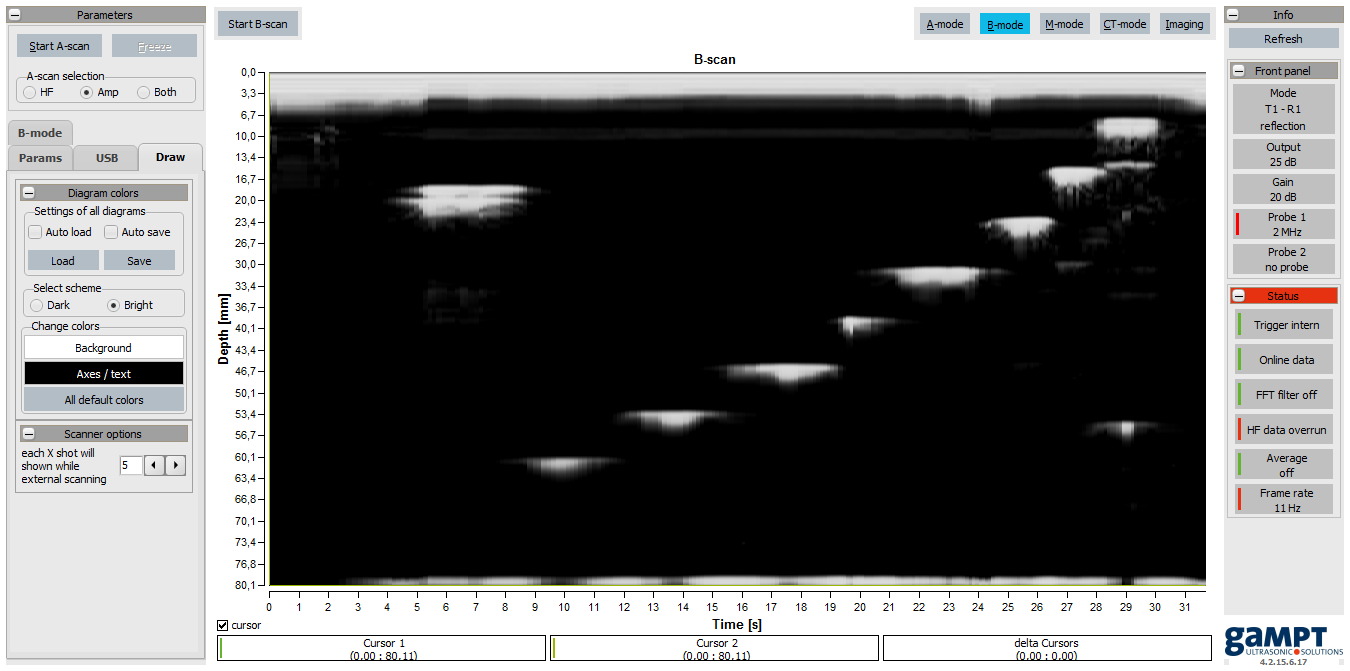
\includegraphics[width=\textwidth]{content/bscan-2mhz_oberseite.png}
  \caption{Messung des Acrylblock von der Oberkante.}
  \label{fig:obs}
\end{figure}
\begin{figure}[H]
  \centering
  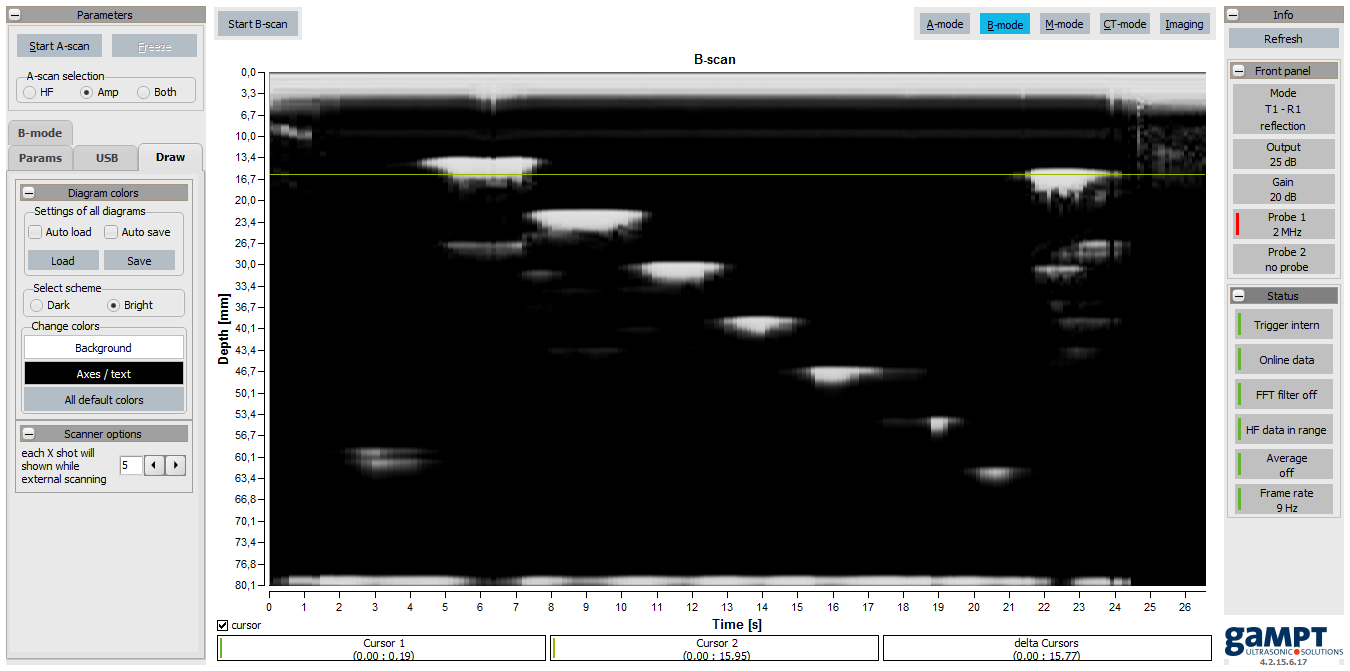
\includegraphics[width=\textwidth]{content/bscan-2mhz_unterseite.png}
  \caption{Messung des Acrylblock von der Oberkante.}
  \label{fig:unts}
\end{figure}
Aus der Aufnahme\ref{fig:obs} und der Aufnahme\ref{fig:unts} können die Bohrungen lokalisiert werden.
Die erhaltenen Werte sind in Tabelle\ref{tab:b-scan} eingetragen.
\begin{table}[H]
    \caption{Messung der Bohrungen mit dem B-Scan .}
    \label{tab:a-scan}
    \centering
    \begin{tabular}{S[table-format=2] S[table-format=2.2(0)e0] S[table-format=2.2(0)e0]  }
        \toprule
        {Bohrung} & {$Oberkante/\si{\milli\meter}$} & {Unterkante$/\si{\milli\meter}$} \\
        \midrule
             1 & 19.98  & 58.85\\
             2 & 18.42  & 60.73\\
             3 & 60.57  & 13.58\\
             4 & 53.08  & 22.32\\
             5 & 45.90 & 30.28\\
             6 & 38.55 & 38.72\\
             7 & 30.91 & 46.36\\
             8 & 23.10 & 54.16\\
             9 & 15.61 & 62.13\\
             10 & 8.12 & / \\
             11 & 55.11 &  15.77\\
        \bottomrule
    \end{tabular}
\end{table}
\noindent
